\documentclass[9pt]{extarticle}

\usepackage[utf8]{inputenc}              % Tipos de caracteres
\usepackage[portuguese]{babel}           % Português
\usepackage[a4paper,portrait]{geometry}  % Tipo de papel
\usepackage{color}                       % Para tratamento da cor
\usepackage{graphicx}                    % Para a imagem
\DeclareGraphicsExtensions{.jpg,.png}
\usepackage{amsmath}                     % Para as matematiquices
\usepackage{amssymb}
\usepackage{array}
\usepackage{gensymb}                     % Grau
\usepackage{multicol}
\setlength{\columnsep}{1cm}
\usepackage{geometry}					% Margens
%\usepackage{xfrac}
\usepackage{colortbl}

\usepackage{multirow}

\addtolength{\topmargin}{-20mm}
\addtolength{\textheight}{55mm}
\addtolength{\oddsidemargin}{-15mm}
\addtolength{\textwidth}{32mm}

\renewenvironment{abstract}
 {\small
  \begin{center}
  \bfseries \abstractname\vspace{-.5em}\vspace{0pt}
  \end{center}
  \list{}{
    \setlength{\leftmargin}{0cm}%
    \setlength{\rightmargin}{\leftmargin}%
  }%
  \item\relax}
 {\endlist}
 
\renewcommand{\abstractname}{Resumo}
%\renewcommand{\bibname}{Referências}

\delimitershortfall-1sp
\newcommand\abs[1]{\left|#1\right|}
\newcommand{\PR}[1]{\ensuremath{\left[#1\right]}}
\newcommand{\PC}[1]{\ensuremath{\left(#1\right)}}
\newcommand{\chav}[1]{\ensuremath{\left\{#1\right\}}}

\newcolumntype{x}[1]{>{\centering\hspace{0pt}}p{#1}}

\begin{document}

\title {\bf \huge T1 - Conversor Termoelétrico}
\author
{{\small Grupo III - João Ferreira (78179) Henrique Rodrigues (78632) Rodrigo C. Carvalho (78646) Cristina Melício (78947)} \\
{\small MEFT - 2ºAno, 2º Semestre - Laboratório de Complementos de Eletromagnetismo e Termodinâmica}}
\date{{\small Sexta-Feira, 13 de Março de 2015}}
\maketitle

\begin{abstract}
\par Nesta experiência foi estudada a emissão de radiação por diversos corpos enquanto aproximação do modelo de Corpo Negro. Verificou-se experimentalmente a Lei de Planck e a Lei de Wien com o auxílio de uma lâmpada de tungsténio para três temperaturas distintas, tendo sido obtido para a constante de Wien o valor de $(2.5\pm0.4)mK$. Posteriormente, determinou-se o expoente da Temperatura na relação de Stefan-Boltzmann, tendo-se verificado que este correspondia a $\alpha(=?\pm?)$. Este expoente foi também analisado para baixas temperaturas através do estudo da face espelhada do Cubo de Leslie, tendo nesse caso sido $\alpha(=?\pm?)$. Por fim, comparam-se as emissividades de diferentes faces do mesmo Cubo de Leslie.
\end{abstract}

\begin{multicols}{2}

\section{Introdução}

\par Esta experiência consiste no estudo de um corpo negro, que é definido como sendo um corpo que absorve toda a radiação que nele incide sem a refletir ou transmitir inteiramente, irradiando posteriormente de acordo com a sua temperatura absoluta $T$.

\par Para um corpo arbitrário define-se o poder de absorção sendo:
\begin{equation}
Q = \frac{P_a}{P_i}
\end{equation}
\begin{center}
\par\noindent {\scriptsize(onde $P_a$ é a potência absorvida e $P_i$ é a potência incidente)}
\end{center}
\par Para o corpo negro tem-se que $Q_N = 1$ uma vez que absorve toda a radiação que nele incide e para os outros corpos tem-se $Q_C < 1$ .
\par A emissividade é dada pelo quociente:
\begin{equation}
e = \frac{Q_C}{Q_N}
\end{equation}
\par Sendo assim, para o corpo negro $e_C = 1$ e para os outros corpos $e_C < 1$.

\par O comportamento de um corpo relativamente à radiação emitida é descrito pelo poder emissivo ou emitância $I_C$ e é caracterizado como sendo a energia radiada por unidade de tempo e por unidade de área em todos os comprimentos de onda. É possível quantificar o poder emissivo do corpo negro $I_N$ pela Lei de radiação de Stefan:
\begin{equation}
I_N = \sigma T^4
\end{equation}  
\begin{center}
\par\noindent {\scriptsize(sendo $\sigma$ a constante de Stefan)}
\end{center}

\par Tem-se assim, o Teorema de Kirchoff que considera a relação entre o poder emissivo e o poder de absorção como sendo:
\begin{equation}
F(T) = \frac{I_C}{Q_C} = \sigma T^4
\end{equation}
\par Deste enunciado, conclui-se que a emissividade e o poder de absorção são iguais, sendo que um bom absorsor é um bom emissor e vice versa.

\par A partir de lei de Stefan, conclui-se que a emissão de radiação por um corpo negro depende apenas da sua temperatura, quando este se encontra em equilíbrio térmico. Tem-se então à Lei de Wien, cujo resultado é quanto maior for a temperatura de um corpo negro menor é o comprimento de onda que ele emite:
\begin{equation}
\lambda_{max} T = b
\end{equation}
\begin{center}
\par\noindent {\scriptsize(onde $\lambda_{max}$ representa o comprimento de onda para o qual o poder emissivo é máximo, e $b$ a constante de Wien)}
\end{center}

\par A relação entre a intensidade da radiação emitida por um corpo negro e a sua temperatura absoluta, $T$, e o seu comprimento de onda, $\lambda$ é dada pela Lei de radiação de Planck:
\begin{equation}
I_{(T,\lambda)} = \frac{2hc^3}{\lambda^5} \frac{1}{e^{\frac{hc}{\lambda k_B T}}-1}
\end{equation}
\begin{center}
\par\noindent {\scriptsize(em que $h$ é a constante de \textit{Planck}, $k_B$ a constante de \textit{Boltzmann} e $c$ a velocidade da luz)}
\end{center}

\par É de realçar ainda que, no que toca ao cubo de Leslie, verifica-se que a diferença de tensão gerada pelo detector seria directamente à intensidade de radiação que sobre ele incide apenas no caso de ele próprio se encontrar a uma temperatura correspondente ao zero absoluto. Todavia, tal não é verdade. De facto, ele irá emitir radiação segundo a lei de Stefan-Boltzmann previamente enunciada. Assim, sabemos que a diferença de potencial gerada será na realidade proporcional à intensidade de radiação emitida pelo detector menos a que sobre ele incide. Sabendo que a temperatura do sensor é quase igual à da temperatura da sala (visto este se encontrar protegido da radiação que sobre ele incide excepto aquando do momento de fazer medições), temos que

\begin{equation}
V \propto (T^4-T_{det}^4)
\end{equation}
\begin{center}
\par\noindent {\scriptsize(em que $V$ é a diferença de potencial medida, $T$ a Temperatura a que se encontra o emissor de radiação e $T_det$ a temperatura do detector)}
\end{center}


\section{Montagem da Experiência}
\subsection{Lei de Planck e Lei de Wien}
\par Na primeira parte da experiência, cujo objetivo é a obtenção do espectro de emissão de um modelo do corpo negro, o esquema da montagem está representado na figura 1.

\begin{center}
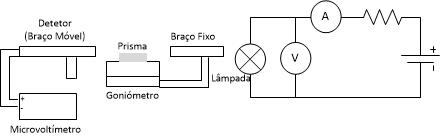
\includegraphics[width=200pt]{parte1.jpg}
\begin{center}
\par\noindent {\scriptsize ({\bf Figura 1}:Esquema da montagem da primeira parte)}
\end{center}
\end{center}

\par O modelo de corpo negro usado para esta parte é uma lâmpada de filamento de tungsténio cuja tensão máxima é $13 V$, sendo, por isso, colocados um voltímetro, em paralelo, e um amperímetro, em série, de forma a controlar a tensão e a corrente no circuito. Além disso, a resistência em série serve para evitar sobrecargas no circuito de alimentação.

\par Tem-se então um goniómetro, associado a um prisma de dispersão, composto por dois braços: o braço fixo que recebe a radiação da fonte e a faz incidir sobre o prisma e o braço móvel que recebe do prisma a radiação refratada e a faz incidir no detetor. O detetor da radiação utilizado é uma termopilha com resposta uniforme na gama compreendida entre os $500 nm$ e os $25000 nm$, ou seja, da radiação verde à infravermelha, que funciona por efeito de \textit{Peltier} devido à diferença de temperatura entre os sensores do início e do fim do detetor.
\par O esquema do prisma de dispersão e dos seus ângulos encontra-se na figura 2.

\begin{center}
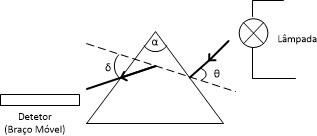
\includegraphics[width=180pt]{prisma.jpg}
\begin{center}
\par\noindent {\scriptsize ({\bf Figura 2}: Esquema do prisma de dispersão)}
\end{center}
\end{center}

\subsection{Verificação da Lei de \textit{Steffan}}
\par Na segunda parte da experiência, retirou-se o goniómetro e o prisma, e colocou-se a uma distância fixa a lâmpada na direção do detetor. O esquema da montagem está na figura 3.

\begin{center}
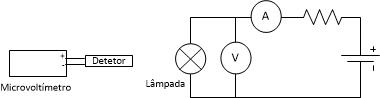
\includegraphics[width=200pt]{parte2.jpg}
\begin{center}
\par\noindent {\scriptsize ({\bf Figura 3}: Esquema da montagem da segunda parte)}
\end{center}
\end{center}

\subsection{Cubo de Leslie}
Na terceira parte da experiência utiliza-se um Cubo de \textit{Leslie} constituído por quatro faces com diferentes revestimentos exteriores. As faces consideradas foram: face preta, face espelhada e duas faces brancas A e B. O esquema da montagem está na figura 4.

\begin{center}
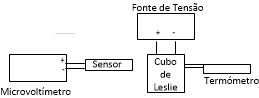
\includegraphics[width=180pt]{parte3.jpg}
\begin{center}
\par\noindent {\scriptsize ({\bf Figura 4}: Esquema da montagem da terceira parte)}
\end{center}
\end{center}


\section{Discussão de Resultados}

\subsection{Lei de Planck e Lei de Wien. Eficiência da lâmpada}

\par Relativamente à primeira parte da experiência, efectuou-se o ajuste experimental dos dados obtidos à lei de Planck. Todavia, verificou-se que os dados apresentavam uma translação em relação ao máximo, fruto de um erro sistemático existente na experiência. Por conseguite, efectuou-se um ajuste do tipo $x-b$ para $(b=150.0\pm23.8)nm$, verificando-se uma muito melhor aproximação dos dados experimentais ao fit efectuado, existindo concordância a nível do máximo em relação ao fit experimental e a previsão teórica (tal como foi apresentado na secção anterior) e apenas começando a verificar-se desvios significativos a partir de cerca de 3000nm. É possível ver a sobreposição dos gráficos para as diversas temperaturas consideradas na figura INSERIR INSERIR.

(IMAGEM DOS TRÊS GRÁFICOS)

\par Subsequentemente, obteve-se um valor para a constante de Wien através do método previamente enunciado. Foi possível obter o seguinte gráfico:

(GRÁFICO DE WIEN)

\par De facto, verificou-se que este correspondia a $B=(\pm)mK$, o qual consequentemente apresenta um desvio à exactidão de $=\%$ e um desvio à precisão de $=\%$. Devemos realçar que, apesar da boa qualidade do valor obtido, esta poderia ser largamente melhorada utilizando um maior número de temperaturas e comprimentos de onda a partir dos quais obter esta constante - de facto, apenas foram estudados 3 pares $\lambda-T$.

\par Relativamente à eficiência da lâmpada, esta foi tomada mediante a integração numérica das curvas obtidas para a Lei de Planck para cada diferente temperatura, tendo-se utilizado o método dos trapézios. Para estimar o erro inerente ao método, integrou-se o erro também mediante o método dos trapézios, obtendo por conseguinte um majorante válido. Assim, foi possível obter os seguintes resultados, tendo em conta que o valor teórico foi previsto pelo software Mathematica:

ARRANJAR ESTA TABELA MERDOSA

\begin{center}
\begin{tabular}{ x{1.5cm},x{1.5cm},x{1.5cm},x{1.5cm},x{1.5cm}}
T(K) & I_{total} & I_{visivel} & $\epsilon($\%$)$ & $\epsilon_t($\%$)$ & \tabularnewline
\hline \hline
$2404 \pm 1$ & $17.7\pm0.12$  & $0.502\pm0.005$  & $2.92\pm0.02$ & $3.9$ &\tabularnewline
$2130\pm1$ & $10.4\pm0.08$ & $0.171\pm0.004$ & $1.64\pm0.04$ &$1.95$ &\tabularnewline
$1886\pm1$ & $6.2\pm0.1$ & $0.048\pm0.004$ & $0.78\pm0.06$$ & $0.84$ & \tabularnewline
\end{tabular}
\par\noindent {\scriptsize (Tabela ?????: Eficiência para diferentes temperaturas)}
\end{center}

\par Além disto foi possível obter o valor da eficiência em função da temperatura mediante a utilização do software Mathematica, ajustada pela equação

\begin{equation}
\epsilon=\frac{\int_0^\infty f(\lambda,T)d\lambda}{\int_{380nm}^{750nm} f(\lambda,T)d\lambda}
\end{equation}

\par Assim, obteve-se um gráfico para a eficiência em função da temperatura, apresentada no seguinte gráfico

GRÁFICO

\par Verificou-se que o máximo ocorreu a $T=7138K$, com um valor de $\epsilon=48.3\%$ pelo que nos encontramos assim aquando da realização da experiência num domínio de eficiências muito baixo. Além disso, notamos que quão menor a temperatura, maior a concordância entre o valor teórico e o valor experimental. Devemos no entanto realçar que existe ainda uma diferença significativa entre a eficiência de um corpoa negro e a da lâmpada, que resulta naturalmente de esta não ser exactamente um corpo negro bem como de ruído inerente à realização da experiência - esta não foi feita na ausência total de luz ambiente, por exemplo.

\subsection{Lei de Stefan}

GRÁFICO STEFAN

\par No gráfico ???? é possível observar os resultados obtidos para esta parte da experiência, tendo-se obtido como valor do expoente na equação de Stefan-Boltzmann o valor $\alpha=??$. De facto, notamos que existe uma discrepância acentuada entre este valor e o expectável teórico, verificando-se um desvio à exactidão de $\%$ e um desvio à precisão de $\%$. Tal resulta naturalmente de isto não ser um corpo negro - como tal, a lâmpada apresenta uma emissividade que varia consoante a temperatura e cuja consequência é induzir um erro progressivo e que se vai aculumando no valor obtido. Além disso, verificamos que no manual do fabricante foi obtido o valor de $??$ para este expoente. Tomando este como valor real, verificamos que existe somente um desvio à exactidão de $\%$ e um desvio à precisão de $\%$, o que indicia uma muito melhor aproximação.

\subsection{Cubo de Leslie}

\par Relativamente ao Cubo de Leslie, estudou-se a emissividade das diversas faces do cubo. Consideraram-se duas temperaturas distintas, tendo-se obtidos os seguintes resultados

(COPIAR TABELA DE LESLIE. ESTOU PREGUIÇOSO).

\par Sabemos que, quanto maior for o valor verificado, de acordo com o Teorema de Kirchoff, mais elevada será a emissividade da face à qual pertence esse valor - sendo que esta será por conseguinte uma melhor emissora de radiação, absorvendo também uma maior quantidade da radiação que sobre ela incide. Assim, pela análise dos resultados, facilmente se depreende que a face com a maior emissividade será a face negra, tal como esperado, e que a de menor emissividade (melhor reflectora) será a espelhada. Todavia, no tocante a ambas as faces brancas, notamos uma discrepância - uma delas apresenta um valor quase idêntico ao da face negra, enquanto que a outra se comporta como esperado e apresenta um valor demarcadamente inferior. Isto é facilmente explicável - uma face branca reflecte a radiação visível. Todavia, nada sabemos quanto à emissividade do material que a constitui no tocante a quaisquer outros comprimentos de onda. Ora, considerando que a zona visível do espectro constituiu uma ínfima parte da emissão da lâmpada - e não aquela para a qual possui o seu máximo de intensidade de emissão - podemos concluir que o material de que esta face é constituída é reflectivo na zona do visível mas possui uma muito elevada emissividade para outras zonas, nomeadamente a do infravermelho. Tal como antecipado, notamos igualmente que quão maior for a temperatura, maior será a intensidade da radiação emitida.

\par Por fim, foi efectuado um processo adicional de medir o valor do expoente da relação de Stefan-Boltzmann, utilizando o raciocínio delineado nos últimos parágrafos da introdução. Assim, verificaram-se os resultados apresentados no seguinte gráfico

GRÁFICO GRÁFICO

\section{Conclusões}

\par Após efectuar a experiência é possível constatar que existem diversos erros associados à execução da própria e que não são elimináveis - interpolação linear dos dados da tabela dos indíces de refracção, ruído electromagnético de fundo, a sensibilidade do aparelho de medição que flutua entre diversos valores de diferença de potencial, entre outros - e que comprometem a qualidade das medições efectuadas, não sendo inteiramente suprimidos pela execução de diversas medidas para cada valor estudado. Todavia, é de notar que os resultados em si se encontram razoáveis, verificando-se que na primeira parte após a translação efectuada existe uma concordância razoável entre os máximos teóricos e experimentais; um valor para a constante de Wien que se encontra dentro da incerteza experimental; um expoente para a Lei de Stefan-Boltzmann que não se afasta demarcadamente daquele obtido pelos fabricantes e, por fim, os resultados previstos teoricamente para o cubo de Leslie. Na parte proposta pelo próprio grupo para a determinação do expoente desta lei a baixas temperaturas foi possível constatar que (:::)

\begin{thebibliography}{9}

\bibitem{guia} Guia de objetivos do trabalho, Professor João Figueirinhas
\bibitem{apontamentos} Apontamentos das aulas teóricas
%\bibitem{site} Wikipedia, the free encyclopedia - Thermoelectric effect. [Online] Available from: \url{http://en.wikipedia.org/wiki/thermoelectric\_effect}
\end{thebibliography}

\vfill

\pagebreak

%\section{Anexos}
%\subsection*{\normalsize Material}
%\begin{itemize}
%\item Cenas
%\end{itemize}
%
%\subsection*{\normalsize Tabelas Completas de Resultados}
%\par Cenas

\end{multicols}

\end{document}

% FOTOGRAFIA
%\begin{center}
%\includegraphics[width=240pt]{NOME SEM EXTENSAO}
%\par\noindent {\scriptsize (Figura X: Descrição)}
%\end{center}

%NOVA SUBSECÇÃO
%\subsection*{\normalsize BLA BLA}

%TABELA
%\begin{center}
%\begin{tabular}{ x{1.5cm} ... }
%i & ... \tabularnewline
%\hline \hline
%1 & 4.15  & 0.15  & 2033 & -  \tabularnewline
%\end{tabular}
%\par\noindent {\scriptsize (Tabela X: Descrição)}
%\end{center}